% !TEX root=/home/tavant/these/manuscript/src/manuscript.tex

\section{PIC simulation results: Boeuf test-case}


  We uses the test-case of Boeuf for three different cases.
  The first is the usual case, without the effects of the radial direction.
  It is expected to return the same results as obtained in \citet{boeuf2018}.
  The two other cases model the effect of the radial direction.
  Two values of the radial length are used\string: $L_R=4\,\centi\meter$ and $2\,\centi\meter$.


  \subsection{Boeuf test-case: Temporal evolution} \label{subsec-temp_boeuf}
  
  \inlinenote{Anne: Donner une table ou faire reference au papier de Thomas pour donner toutes les caracteristiques de tes simulations
  Si quelqu un essaie de refaire tes calculs de these, on doit avoir les informations pour les refaire ;-) }

  Since the ionization source term is constant in this test-case, a steady state is reached after a 6 or $8\micro\second$.
  \Cref{fig-boeuf-temporal} presents the temporal evolution of the mean plasma density and temperature.
  We see that when the radial direction is modeled, the density and the mean electron temperature and the radial electron temperature is reduced, as expected when increasing the losses with a constant ionization source term.

  \renewcommand\subfigurewidth{0.49\textwidth}

  \begin{figure}[hbtp]
    \centering
    \begin{tabular}{cc}
      \subfigure{Boeuf_ne_temporal}{a}{20,20} &
      \subfigure{Boeuf_Te_temporal}{b}{20,20} \\
    \end{tabular}
    \caption{({\bf a}) temporal evolution of the mean plasma density and  ({\bf b})  temporal evolution of the  electron temperatures obtained with three different radial models for the simulation case of Boeuf. }
    \label{fig-boeuf-temporal}
  \end{figure}

  We see on \cref{fig-boeuf-temporal}.{\bf b} that the radial temperature remains constant when the radial direction is not modeled.
  This is due to the fact that the collisions are not modeled in the simulations, so that there is not momentum and energy transfer possible from the axial and azimuthal directions, and the radial direction.

  However, we know from the radial-azimuthal simulations that there is a transfer, resulting in a plasma less anisotropic than observed here.
  This aspect is discussed in \cref{subsec-MCC_boeuf,subsec-radial-heating}.
  With the radial losses, the radial temperature decreases from the initial temperature $\Te=5\,\volt$ to $\Te_R\simeq 2.2$ and $ 3.3\,\volt$ for $L_R=2$ and $3\,\centi\meter$, respectively.
  The total temperature $\Te$ shows a similar decrease with the increase of the radial losses.

  \subsection{Boeuf test-case: Axial profiles} \label{subsec-axial_boeuf}

  \Cref{fig-boeuf_axialone,fig-boeuf_axialtwo}  show the axial profile at steady-state of several plasma quantities.
  The variables are averaged in the azimuthal direction and in time between $t=8$ and $t=10\,\micro\second$.
  The results  obtained with three different radial models for the simulation case of Boeuf are overlaid.
  \cref{fig-boeuf_axialone}.{\bf a} shows the axial electric field $E_z$.
  The differences in $E_z$ are small, but we can still distinguish that the amplitude of $E_z$ is reduced with the increased radial losses.
  The electron density $n_e$ shown in \cref{fig-boeuf_axialone}.{\bf b} is almost not affected, except in for $z>1\,\centi\meter$, where the electron losses at the wall can be seen.

  \begin{figure}[hbtp]
    \centering
    \begin{tabular}{cc}
      \subfigure{Boeuf_electric_field}{a}{30,22} &
      \subfigure{Boeuf_ne_axial}{b}{30,24} \\
    \end{tabular}
    \caption{Averaged axial profiles at steady state of ({\bf a}) the axial electric field $E_z$, ({\bf b}) the mean plasma density obtained with three different radial models for the simulation case of Boeuf. }
    \label{fig-boeuf_axialone}
  \end{figure}

  On the other hand, the axial electron density current $J_{e, z}$ (\cref{fig-boeuf_axialtwo}.{\bf a}) and the electron temperature (\cref{fig-boeuf_axialtwo}.{\bf b}) are significantly reduced when the radial losses are modeled.
  We see a factor of two on $J_{e, z}$ between the case $L_R=2\,\centi\meter$ and the case without losses.
  However, we have seen that the electron density is almost unaffected.
  This means that the electron axial velocity is reduced, because of the radial losses.

  \begin{figure}[hbtp]
    \centering
    \begin{tabular}{cc}
      \subfigure{Boeuf_Je_axial}{a}{30,22} &
      \subfigure{Boeuf_Te_axial}{b}{25,80} \\
    \end{tabular}
    \caption{Averaged axial profile at steady state of ({\bf a})  the axial electron current density $J_{e, z}$, and ({\bf b}) the  electron temperature obtained with three different radial models for the simulation case of Boeuf. }
    \label{fig-boeuf_axialtwo}
  \end{figure}


  We see that the electron transport is highly affected.
  This is expected to be due to the reduced electron temperature, which reduces the amplitude of the instability at saturation.
  It is confirmed by the values presented in \Cref{fig-boeuf-instability}.
  \cref{fig-boeuf-instability} shows on the left the average standard deviation of the azimuthal electric field.
  It represents the amplitude of the oscillation.
  We casee that the amplitude of the instability is significantly affected by the electron radial losses.

  \begin{figure}[hbtp]
    \centering
    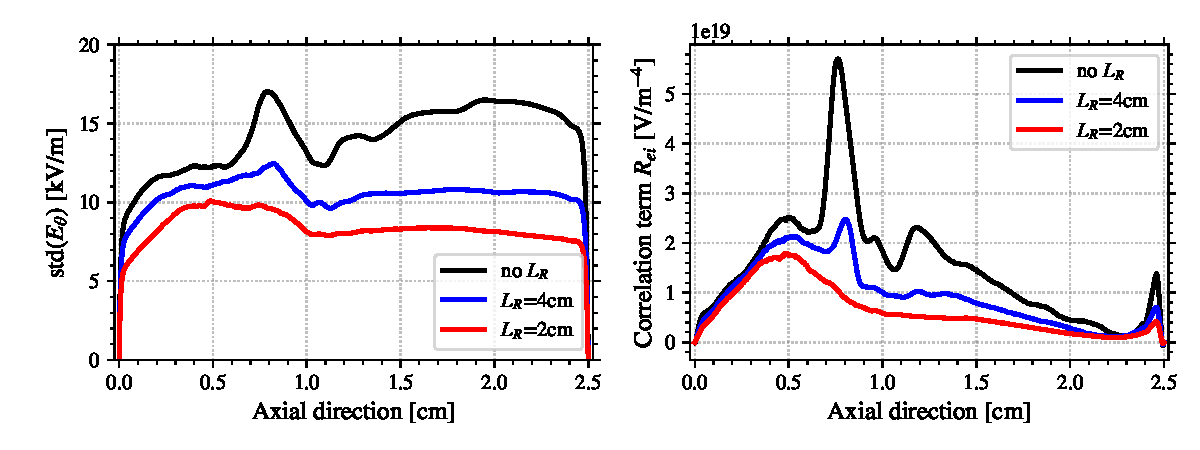
\includegraphics[width=\textwidth]{Boeuf_instability_characteristics}
    \caption{Axial profiles of the characteristics of the instability, (left) average of the standard deviation of the azimuthal electric field, (right) electron-ion friction force calculated by the correlation between $n_e$ and $\Te$.    }
    \label{fig-boeuf-instability}
  \end{figure}

  On the right panel of \cref{fig-boeuf-instability} we see the correlation term
  \begin{equation} \label{eq-rei}
    R_{ei} = < n_e E_{\theta} >
  \end{equation}
  responsible for the electron axial enhanced transport.
  Again, we see a decrease on the amplitude of $R_{ei}$ because of the reduced oscillation amplitude.


  \subsection{Boeuf test-case with collisions} \label{subsec-MCC_boeuf}
  % Script on Juno (CH-6_Boeuf)

  We have seen that because there is no collision in the test-case of Boeuf, there is no energy transfer toward the radial direction.
  Thus, we investigate here the impact of the neutrals on the electron anisotropy by modeling the collisions with the \ac{MCC} algorithm.

  The xenon neutrals are injected at the anode side with density of $n_g=\sn{1}{17}\,\meter$${-3}$, an axial velocity $v_g = 200 \,\meter\per\second$ and a temperature $T_g=640\,\kelvin$.
  We model the neutral flow with the continuity and momentum conservation equation, while keeping their temperature constant.
  The ionization source term used to sustain the plasma is a loss term in the continuity equation.
  \Cref{fig-boeuf-neutrals} shows the neutral density and velocity obtained at steady-state.

  \begin{figure}[hbtp]
    \centering
    \begin{tabular}{cc}
      \subfigure{boeuf_MCC_ng}{a}{20,20} &
      \subfigure{boeuf_MCC_vg}{b}{20,15} \\
    \end{tabular}
    \caption{Axial profile at steady-state ($t=14\,\micro\second$) of ({\bf a}) the neutral density and  ({\bf b})  the neutral axial velocity, for  simulation case of Boeuf with the electron-neutral scattering. }
    \label{fig-boeuf-neutrals}
  \end{figure}
  We see in \cref{fig-boeuf-neutrals} that the neutrals are significantly depleted because of the forced ionization source term.
  The neutral density gradient accelerates the neutrals in the axial direction by a factor of two, which reduces even more the neutral density.
  Thus, the electron-neutral scattering will be significant on the anode side of the chamber.

  \begin{figure}[hbtp]
    \centering
    \begin{tabular}{cc}
      \subfigure{boeuf_mean_Te}{a}{20,20} &
      \subfigure{boeuf_mean_Tez_profile_MCC}{b}{20,15} \\
    \end{tabular}
    \caption{({\bf a}) temporal evolution of the electron kinetic energy in the three directions and  ({\bf b}) axial profile of the electron temperature at steady state obtained for the simulation case of Boeuf with the electron-neutral scattering. }
    \label{fig-boeuf-temporalMCC}
  \end{figure}

  \Cref{fig-boeuf-temporalMCC} shows the temporal evolution of the mean electron kinetic energy on the left, and on the right it shows the axial profile of the electron temperatures, decomposed on the three directions.
  We see that they is a small transfer of energy between the radial direction and the others.
  In particular, close to the anode where the gas density is high, the radial and axial temperatures decrease below the initial temperature $\Te_{, inj}=5\,\volt$.
  In contrast, at the maximum of the magnetic field where the gas density is low (and then electron neutral scattering is considered to be negligible), the radial energy increases to $\Te_R=7\,\volt$.
  However, the anisotropy stays significant, compared to the  radial-azimuthal simulations presented in \cref{ch-2}.

  \subsection{Radial heating of electrons} \label{subsec-radial-heating}
  The large anisotropy observed in \Cref{fig-boeuf-temporal,fig-boeuf-temporalMCC}, compared to the results of \cref{ch-2} might be due to the difference on neutral density.
  However, the collisions are usually neglected in \ac{HET}s compared to the instability.
  Hence, the plasma fluctuations may be responsible for the electron radial heating.

  The electron power gain is due to Joule heating
  \begin{equation} \label{eq-epower}
      \vect{P_{\rm J}} = \vect{J_e} \cdot \vect{E},
  \end{equation}
  with $\vect{J_e}$ the electron density current and $\vect{E}$ the electric field.
  \Cref{fig-epower_radialone} shows the radial profiles of the electron (and ion) current density $< J_{e, R}>$ and the radial electric field $ < E_R >$, averaged in the azimuthal direction.
  The current density increases linearly with the radial position.
  This is due to the artificial uniform injection of particles that compensates the radial losses (see \cref{sec-bidimentionnal_simulation} for more details).


  \begin{figure}[hbtp]
    \centering
    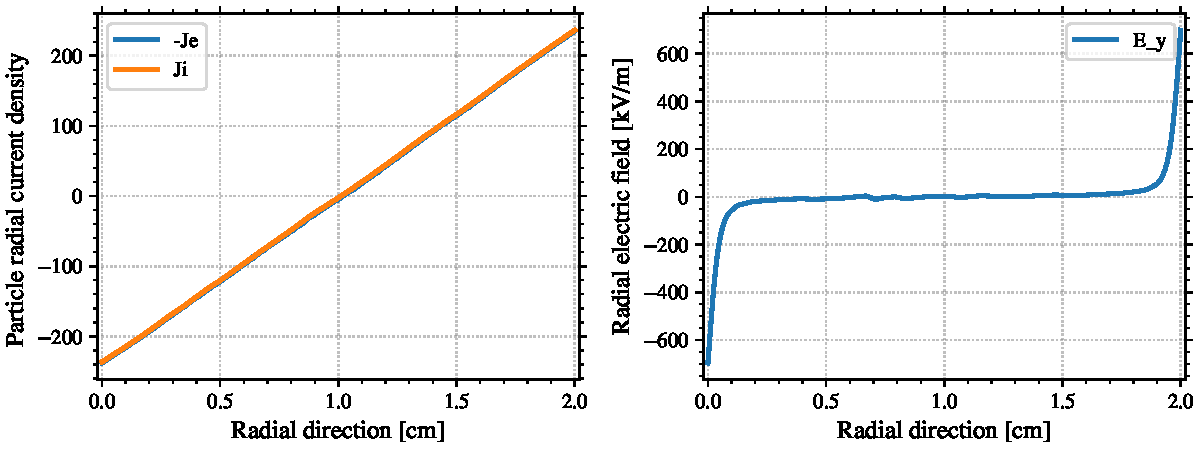
\includegraphics[width=\textwidth]{R_joule_heating_one}
    \caption{Radial profiles averaged in the azimuthal direction of (left) the electron and ion current densities and (right) radial electric field in the radial-azimuthal \ac{PIC} simulation presented in \cref{ch-2}. }
    \label{fig-epower_radialone}
  \end{figure}

  \Cref{fig-epower_radial} shows the mean Joule heating in the radial direction $\bar{P_{\rm J, R}} = < J_{e, R} E_R >$, and the product of the mean quantities $< J_{e, R}>  < E_R >$.
  The product $< J_{e, R}>  < E_R >$ is close to zero , except in the sheaths.

  \begin{figure}[hbtp]
    \centering
    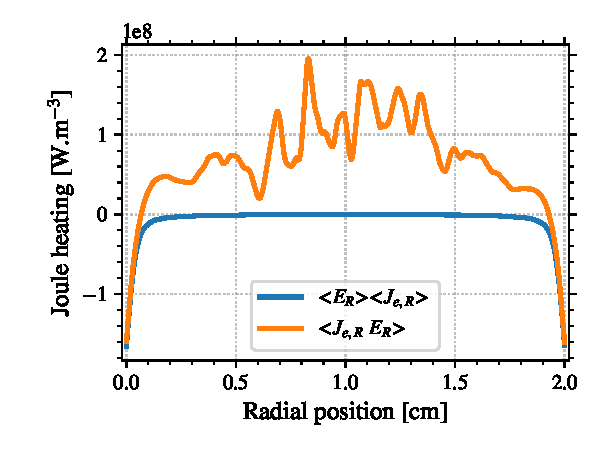
\includegraphics[width=\defaultwidth]{R_joule_heating_two}
    \caption{Electron power gain in the Radial-azimuthal }
    \label{fig-epower_radial}
  \end{figure}

  We see that the mean Joule heating $\bar{P_{\rm J, R}}$ is not zero in the center of the simulation, while the product of the mean is zero.
  Indeed, the mean electric field in the bulk is almost zero.
  This means that there is an energy transfer to the radial direction of the electrons due to the correlation between $\vect{J_e}$ and $\vect{E}$.
  For this energy transfer to be present, the radial direction needs to be resolved.

  A similar radial heating has been observed by \citet{heron2013}.
  The authors observe no heating when the instability was only perpendicular to the magnetic field, as it is in a \ac{1D} or a \ac{2D} axial-azimuthal simulation.
  However, when the direction parallel to the magnetic field is resolved, the electrons are heated, but the physical mechanism remains unclear.
  In \citet{janhunen}, the authors observe a similar radial heating of the electrons, but due to the presence of a \ac{MTSI}.
  As discussed previously, we do not observe the \ac{MTSI} in our simulation, meaning that it has to be due to another mechanism.


  \subsection{Electron azimuthal drift velocity} \label{subsec-drift}

  We showed in \cref{ch-5} that the instability growth rate is proportional to the electron azimuthal drift.
  In the radial-azimuthal simulation, the drift was only due to the $\vect{E} \times \vect{B}$ drift
  \begin{equation} \label{eq-exbdrift}
    u_{E \times B} = - \frac{E_z}{B_r}
  \end{equation}

  \Cref{fig-Jetheta_sum} shows the axial profile of the azimuthal electron mean velocity $u_{e, \theta}$ at steady-state ($t = 14\,\micro\second$) for the case without the radial losses modeled.
  The drift velocity $u_{E \times B}$ is also shown.
  We can see that the electron velocity is no more equal to the $u_{E \times B}$ drift.
  Instead, we saw in \cref{fig-boeuf_axialtwo} that the electron density presents a large axial gradient.
  This leads to the diamagnetic drift
  $$u_{\rm Dia}=\frac{\nabla_z (n_e {\rm T}_{e,z})}{n_e B_r}.$$
  The value of the diamagnetic can be seen in \cref{fig-Jetheta_sum}.


  \begin{figure}[hbtp]
    \centering
    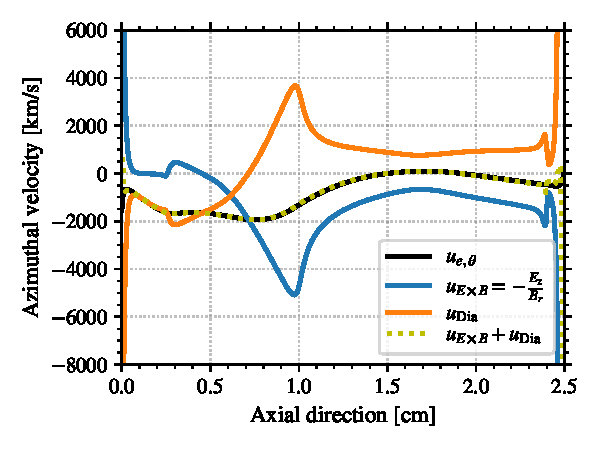
\includegraphics[width=\defaultwidth]{Boeuf_Je_x_axial_one}
    \caption{Axial profile of the electron azimuthal velocity, the $\vect{E} \times \vect{B}$ drift velocity and the diamagnetic velocity and some of the $\vect{E} \times \vect{B}$ and diamagnetic velocities at steady state for the simulation test-case of Boeuf without radial losses.}
    \label{fig-Jetheta_sum}
  \end{figure}


  We see that $u_{\rm Dia}$ is of the same order of magnitude as $u_{E \times B}$, but of the opposite sign.
  Moreover, we see that we have 
  $$ u_{e, \theta} =   u_{E \times B} + u_{\rm Dia}$$
  everywhere in the simulation domain.
  \Cref{fig-Jetheta} shows the values of $ u_{e, \theta},   u_{E \times B}$, and $u_{\rm Dia}$ for the three cases.
  We can see that the magnitude of $u_{e, \theta} $ decreases when the radial losses are present.
  However, the amplitude of both $u_{\rm Dia}$ and $u_{E \times B}$ decreases as well.

   
  \begin{figure}[hbtp]
    \centering
    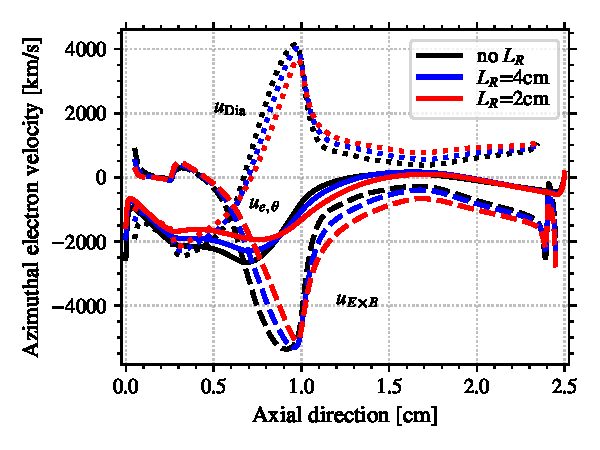
\includegraphics[width=\defaultwidth]{Boeuf_Je_x_axial}
    \caption{Axial profile of the electron azimuthal velocity, the $\vect{E} \times \vect{B}$ drift velocity and the diamagnetic velocity at steady state with three different radial models for the simulation test-case of Boeuf. The sheaths (close to the axial boundaries) are removed from the figure to ease the reading.}
    \label{fig-Jetheta}
  \end{figure}

